\documentclass{article}
\usepackage{tikz}

\begin{document}

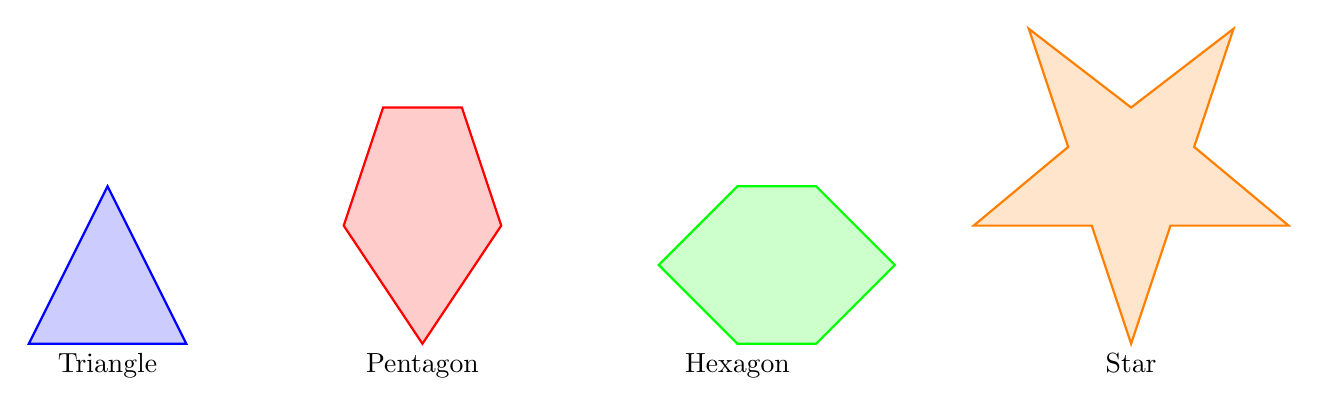
\begin{tikzpicture}[scale=1]

  % --- Triangle (manual path) ---
  \draw[blue, thick, fill=blue!20] (0,0) -- (2,0) -- (1,2) -- cycle;
  \node[below] at (1,0) {Triangle};

  % --- Pentagon (manual path) ---
  \draw[red, thick, fill=red!20] 
    (5,0) -- (6,1.5) -- (5.5,3) -- (4.5,3) -- (4,1.5) -- cycle;
  \node[below] at (5,0) {Pentagon};

  % --- Hexagon (manual path) ---
  \draw[green, thick, fill=green!20] 
    (9,0) -- (10,0) -- (11,1) -- (10,2) -- (9,2) -- (8,1) -- cycle;
  \node[below] at (9,0) {Hexagon};

  % --- Star (manual path) ---
  \draw[orange, thick, fill=orange!20]
    (14,0) -- (14.5,1.5) -- (16,1.5) -- (14.8,2.5) -- (15.3,4)
    -- (14,3) -- (12.7,4) -- (13.2,2.5) -- (12,1.5) -- (13.5,1.5) -- cycle;
  \node[below] at (14,0) {Star};

\end{tikzpicture}

\end{document}
